\documentclass{beamer}
\usepackage[ngerman]{babel}
\usepackage{comment}
\usepackage{nameref}

\usetheme{Warsaw}
\usecolortheme{seahorse}



\title{Entwicklung eines Moduls zur Umstellung von direkten Datenbankzugriffen zu einer gekapselten Datenbankkommunikation mit optionaler Simulationsmöglichkeit}
\author{Frank Loleit}
\institute{Fachinformatiker (Anwendungsentwicklung)}
\titlegraphic{
\includegraphics[scale=0.2]{argusLogo.png}}
\date{\today}



\defbeamertemplate*{footline}{infolines theme}
{
  \leavevmode%
  \hbox{%
  \begin{beamercolorbox}[wd=.333333\paperwidth,ht=2.25ex,dp=1ex,center]{author in head/foot}%
    \usebeamerfont{author in head/foot}\insertshortauthor%~~(\insertshortinstitute)
  \end{beamercolorbox}%
  \begin{beamercolorbox}[wd=.333333\paperwidth,ht=2.25ex,dp=1ex,center]{title in head/foot}%
    \usebeamerfont{title in head/foot}Argus Data Insights
  \end{beamercolorbox}%
  \begin{beamercolorbox}[wd=.333333\paperwidth,ht=2.25ex,dp=1ex,right]{date in head/foot}%
    \usebeamerfont{date in head/foot}\insertshortdate{}\hspace*{2em}
    \insertframenumber{} / \inserttotalframenumber\hspace*{2ex}
  \end{beamercolorbox}}%
  \vskip0pt%
}

\setbeamertemplate{blocks}[rounded][shadow=false]
\setbeamercolor{block body}{bg=white}
\setbeamercolor{block title}{bg=white, fg=blue}

\makeatletter
\newcommand*{\currentname}{\@currentlabelname}
\makeatother

\begin{document}



\begin{frame}
\titlepage
\end{frame}

\begin{frame}
    \frametitle{Inhalt}
    \tableofcontents
\end{frame}

\section{Einleitung}
    \subsection{Herangehensweise und Ziele}
    
        \begin{frame}{Ausgangsüberlegung}
            \begin{definition}{Customer Obsession}
                    
            \end{definition}
        \end{frame}
        
        
        
        \begin{frame}{\insertsectionnumber\space \currentname}
            \begin{figure}[htp]
                \centering
                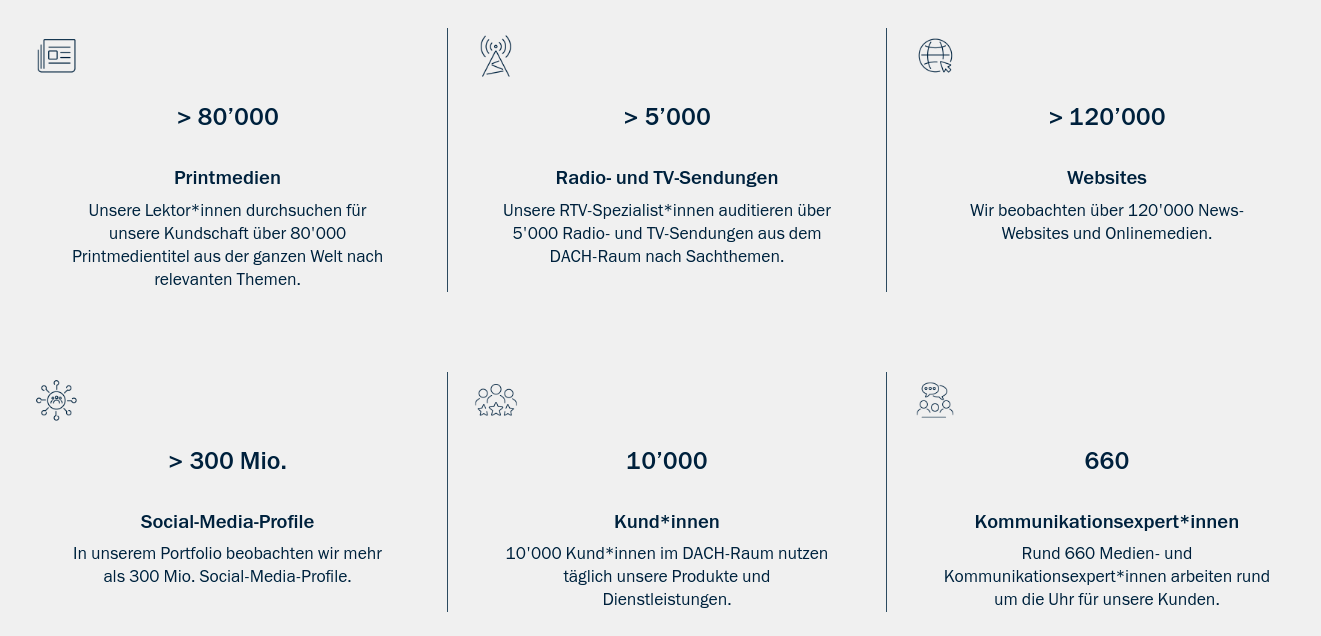
\includegraphics[scale=0.23]{ArgusProfil.png}
                \caption{Portfolio}
                \label{fig:my_label}
            \end{figure}
        \end{frame}
        
    \subsection{Argus Data Insights}
    
        \begin{frame}{Unternehmensprofil von Argus}
            \begin{figure}[htp]
                \centering
                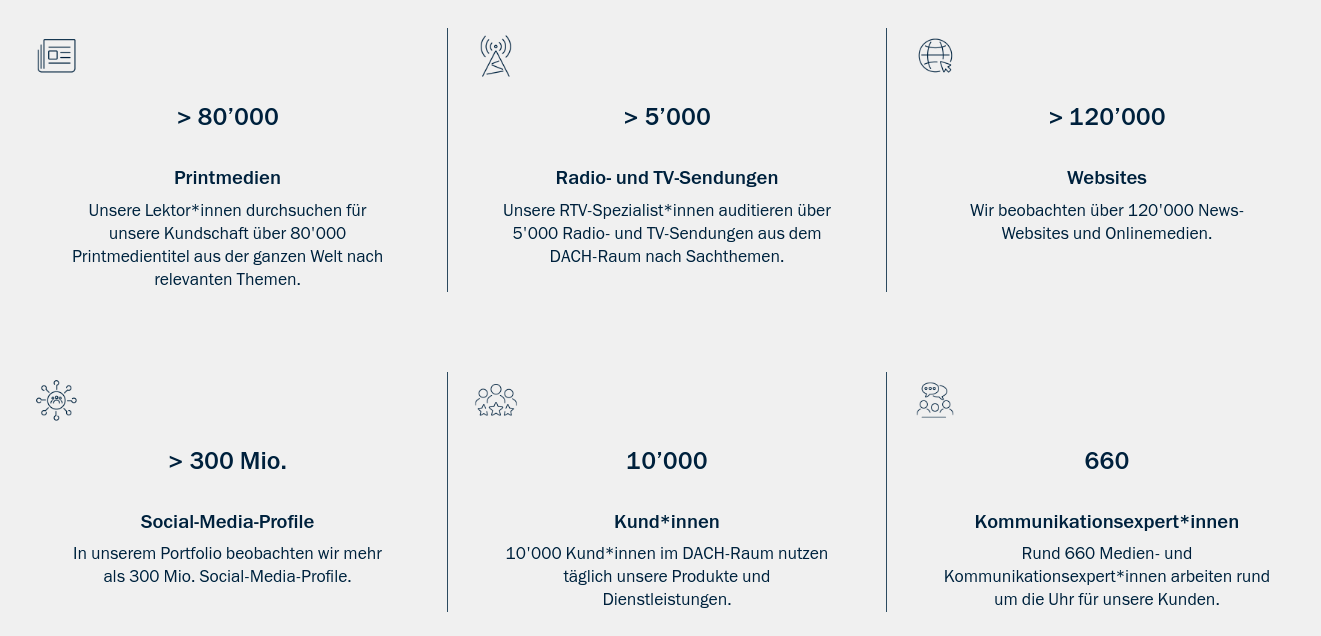
\includegraphics[scale=0.23]{ArgusProfil.png}
                \caption{Portfolio}
                \label{fig:my_label}
            \end{figure}
        \end{frame}            
        
        \begin{frame}{\insertsectionnumber\space \currentname}
            \begin{block}{Architektur}
                Die Desktop-Applikation \glqq Arche\grqq{} stellt Funktionen zur Digitalisierung und Aufbereitung von Medien bereit.
            \end{block}
            \begin{block}{Datenbankkommunikation}
                Um die Kommunikation zwischen .NET und SQL zu gewährleisten, stehen hartkodierte Queries in Persistence-Klassen bereit.
            \end{block}
        \end{frame}
                
            
            
            
           
            
        

\end{document}